\documentclass{ximera}
\input{../preamble.tex}

\author{D. Davis \and R. Speckert \and N. Shay \and A. Davis}
\title{Measurement, Data Collection and Represenatation} \license{CC BY-NC-SA 4.0}
\begin{document}

\begin{abstract}
\end{abstract}
\maketitle

\begin{onlineOnly}
\section*{Measurement, Data Collection and Represenatation}
\end{onlineOnly}

\subsection*{Units}
When collecting and recording data, be sure to always include the correct units.  Also, the units must make sense to the magnitude of the data.  For example, if you were to measure the width of the room in which you are seated, the most logical SI units would be meters and the most logical measuring device would be a meter stick or tape measure.  
Why not record the width of the room in millimeters?  
Recording measurements in units that are logical helps with visualization of the actual size.  
Also, know when the unit is linear, squared, or cubed.   Check these images (not to scale):

\begin{center}
\tdplotsetmaincoords{70}{130}
	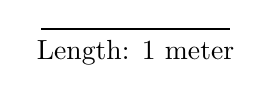
\begin{tikzpicture}[scale=0.6]
\draw[line width=1pt](0,0,0)--(4,0,0) ;
\node[] at (2, -0.5, 0)   {Length: $1$ meter};
     \end{tikzpicture}\quad\quad
         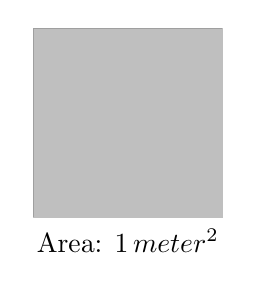
\begin{tikzpicture}[scale=0.6]
\filldraw[gray, opacity=0.5] (4,4,0)--(0,4,0)--(0,0,0)--(4,0,0)--cycle;
\node[] at (2, -0.5, 0)   {Area: $1\, \text{meter}^2$};
	\end{tikzpicture}\quad\quad
	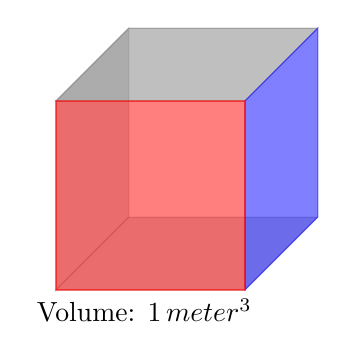
\begin{tikzpicture}[scale=0.6]
   \filldraw[gray, opacity=0.3](0,0,2)--(0,4,2)--(0,4,-2)--(0,0,-2)--cycle;
   \filldraw[gray, opacity=0.3] (4,0,2)--(0,0,2)--(0,0,-2)--(4,0,-2)--cycle;
   \filldraw[gray, opacity=0.5] (0,4,2)--(0,4,-2)--(4,4,-2)--(4,4,2)--cycle;
   \filldraw[blue, opacity=0.5] (4,4,2)--(4,4,-2)--(4,0,-2)--(4,0,2)--cycle;
   \filldraw[red, opacity=0.5] (0,4,2)--(4,4,2)--(4,0,2)--(0,0,2)--cycle;
   \node[] at (1.1, -1.2, 0)   {Volume: $1\, \text{meter}^3$};
\end{tikzpicture}
%    \end{center}     
\end{center}

\begin{question}
    For each example, select an appropriate type of measurement.

    John lives in an $1,800$ sq. ft. house: \wordChoice{\choice{Length}, \choice[correct]{Area},\choice{Volume}}

    Sarah purchases $5$ gallons of paint: \wordChoice{\choice{Length}, \choice{Area},\choice[correct]{Volume}}
\end{question}

\begin{warning}
\begin{itemize}
    \item Units are as important to a measured value as the number. Always include units when recording a measurement. 
\item Make sure the units make sense. For example, don’t give the length of a typical pencil in meters—instead give the dimension in centimeters or millimeters.
\end{itemize}
\end{warning}

 \subsection*{Units Conversion}

 \subsection*{Measurement Process}
 Technicians measure stuff. Therefore, it is important to report a measurement in a meaningful and reliable format.
To do this, the technician must:
\begin{itemize}
\item Select the correct instrument and be knowledgeable of how it works and how to care for it.
\item Calibrate the instrument (transfer standards are traceable to \href{https://www.nist.gov/}{NIST} or other sources).
\item Report  measurement accurately, to a meaningful level of precision, and with proper units.
\end{itemize}

When measuring the thickness of a metal layer resulting from a chemical vapor deposition (CVD), a technician would use a scanning electron microscope \href{https://www.nist.gov/news-events/news/2023/05/leveling-sem-measurements-chip-manufacturing}{(SEM)}.  A SEM is a high precision, delicate instrument that requires training on how to use, care for, and calibrate the device. Many other measuring instruments are used in manufacturing including micrometers, calipers, hardness and surface testers, gauges, and more. 

The accuracy of a measuring instrument is the ability to yield the true or correct value and the precision is the ability to repeat values with small variation. For measuring instruments to be accurate and precise, they must be used correctly, handled and cared for properly, and calibrated. 

Calibration of measuring instruments is crucial to the measurement process. The calibration requirements vary by instrument and applications. Sometimes calibration might be as simple as checking or zeroing the instrument while some instruments used is critical measurement processes may require periodic calibration using standards or transfer standards from the National Institute for Science and Technology (NIST).
    
The degree of precision in reporting a measurement is limited by the least precise measuring instrument used in the process. 
\begin{question}
When measuring the width of the room you are in, suppose you used the balsa wood meter stick given to you at the local bank for opening a new account.  When you got near the wall, you pull out the engineer’s scale calibrated to millimeters and report the width of the room to the nearest millimeter.  Is that level of precision valid?  Discuss why or why not?   So how strong is a chain?  A chain is as strong as the weakest link just like a measurement can be no more precise than the least precise measuring instruments used in the process. 
\end{question}

\begin{question}
When recording a measurement, we write the numeric value to the level of decimal points used in the measurement and include units. Are the following measurements equal?  Explain your answer.   
$$20\text{cm}\quad 20.0\text{cm}\quad 20.00\text{cm}\quad 20.000\text{cm} $$

\begin{multipleChoice} 
\choice{Yes, $20=20.0=20.00=20.000$.} 
\choice{No, (insert silly reason here)} 
\choice[correct]{No, (insert a good reason here)}
\end{multipleChoice} 
\end{question}



 
\begin{exploration}\label{exp:histogram1}
Consider a sample of 100 silicon wafers whose thickness of a metal layer resulting from a chemical vapor deposition (CVD) in a semiconductor plant. The data represent the layer thickness on semiconductor wafers measured in angstroms (one ten billionth of a meter).

% \begin{pdfOnly}
% Access GeoGebra interactives through the online version of this text at 

% \href{https://ximera.osu.edu/qcstats}{https://ximera.osu.edu/qcstats}.
% \end{pdfOnly}
CLICK on the SLIDER to change the number of buckets (bars).

\begin{onlineOnly}
\begin{center} 
\geogebra{dhvgryen}{800}{600} 
\end{center}
\end{onlineOnly}

We can see by the histogram output that the data has the triangular shape and symmetry associated with the bell shape. We can say that this sample data is normally distributed.


\end{exploration}

I'm including this wafer pic just for fun:

\begin{image}
         \includegraphics[height=1.5in]{200mmWafer.png}
\end{image}


\section*{Practice Problems}

\section*{References}
Wafer photo credit: \textit{Processed 200 mm Si Wafer} by Goldenvu CC BY-SA 4.0.

\end{document} 